\documentclass{article}
\usepackage{amsmath}
\usepackage[utf8]{inputenc}
\usepackage{graphicx}
\usepackage{tikz}
\usetikzlibrary{shapes.geometric, positioning}

\begin{document}

\begin{center}
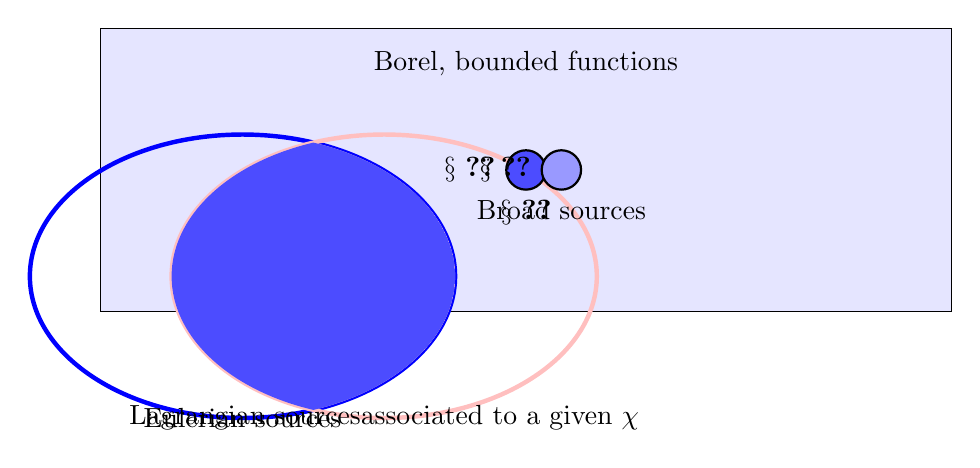
\begin{tikzpicture}[scale=0.9]
    \draw[fill=blue!10] (-6,-2) rectangle (6,2);
    \node at (0,1.5) {Borel, bounded functions};
    
    \draw[ultra thick, blue] (-4,-1.5) ellipse (3 and 2);
    \node at (-4,-3.5) {Eulerian sources};
    
    \draw[ultra thick, pink] (-2,-1.5) ellipse (3 and 2);
    \node at (-2,-3.5) {Lagrangian sources \\ associated to a given $\chi$};
    
    \node [circle, draw, thick, minimum size=0.5cm, fill=blue!70, label={below:$\S~$\ref{sec:nonsmooth}}, label=left:$\S~$\ref{sec:smooth}] at (0,0) {};
    \node [circle, draw, thick, minimum size=0.5cm, fill=blue!40, label={below:Broad sources}, label=left:$\S~$\ref{sec:broad}] at (0.5,0) {};
    
    \path[clip] (-4,-1.5) ellipse (3 and 2);
    \fill[pink!70] (-2,-1.5) ellipse (3 and 2);
    \node [circle, draw, thick, minimum size=0.5cm, label=left:$\S~$\ref{sec:smooth}] at (0,0) {};
    
    \path[clip] (-2,-1.5) ellipse (3 and 2);
    \fill[blue!70] (-4,-1.5) ellipse (3 and 2);
    \node [circle, draw, thick, minimum size=0.5cm, label=above:$\S~$\ref{sec:nonsmooth}] at (0.5,0) {};
    
\end{tikzpicture}
\captionof{figure}{Relations among the sources determined for a fixed continuous solution of the balance law~\eqref{EE} under the non-degeneracy Assumption~\eqref{ass:h}. When the Lagrangian source is continuous, it is `the' source term in all the formulations.}
\label{fig:relations}
\end{center}

\end{document}